% Chapter Template

\chapter{Conclusions}\label{Chapter7} 

Searches for heavy neutral leptons in events with three charged leptons, either from a common vertex or with two leptons forming a displaced vertex. The public
results can be found in References~\cite{Sirunyan:2018mtv} and~\cite{CMS-PAS-EXO-20-009}, respectively.\\

\section{Summary}
The observation of neutrino flavor oscillations was one of the first 
definite experimental indications of the
presence of new physics not described by the SM theory. 
Thus, the comprehension of the mechanism behind the neutrino masses would be an essential guide for the development of new BSM physics models. Therefore, it is crucial for the LHC experiments to investigate the signatures of all possible neutrino mass models to try spotting the mysterious new physics.\\
The two results presented in this thesis cooperate in the arduous attempt of confronting exotic BSM
models with the experimental data. The aspiration is to find new
particles able to describe the unexplained
physics observations not covered by the SM. 

Our studies focus on the concept of right-handed (RH) neutrinos as
implemented in heavy neutral lepton (HNL) models. The introduction of massive RH
neutrinos provides an answer to the SM problem of the
neutrino masses via the seesaw mechanism.  
In Chapters~\ref{Chapter1} and~\ref{Chapter3}, we illustrated
the relevance and the interest for the
ongoing HNL search program, describing first the theory setting 
and then mentioning the various experiments and results
focusing on HNL signatures.\\
When we hypothesize new particles as RH neutrinos, N$_{I}$, we
are interested in their properties like the mass $M_I$ and
their mixing parameter, $|V_{\alpha I}|^2$,  with the SM neutrino of flavor $\alpha$,
related to the Yukawa coupling $F_{\alpha I}$. The values of $|V_{\alpha
  I}|^2$ are unknown. The measured experimental
sensitivities are expressed in
terms of the coupling $|V_{\alpha I}|^2$
as a function of $M_I$ for a given flavor $\alpha$. 

Furthermore we introduced a list of direct HNL search results; we give an overview
of the past and current experimental landscape describing the different decay modes and
mass ranges that are targeted by the single measurements.
The strategies adopted in direct HNL searches vary greatly with the mass range under investigation. For $M_{I} > 5$\GeV, \hnl can be
produced uniquely at high-energy particle colliders like the LHC, via
different possible 
mechanisms (vector boson fusion, s-channel exchange of virtual
W-bosons or in real gauge boson decays) according to the production
energy and \hnl mass. For $M_{I} < 5$\GeV, we recur to b-factories
or fixed target experiments. \\
Special attention is paid to lepton and hadron collider
searches. The LEP results from DELPHI provide the best results at low mass from collider experiment up to the publication of the results
of this dissertation. The outstanding sensitivity at low mass from
$e^{+}e^{-}$ data was surely a good motivation to invest into extending the low mass sensitivity of
the CMS experiment as well.\\

Chronologically, we have focused first on the
moderate and high mass search and then migrated to the very low mass search which
necessarily requires the inclusion of scenarios with displace decays.

During my first PhD year, I worked on the ``search for heavy neutral leptons in events with three charged
 leptons in proton-proton collisions at $\sqrt{s}$ =
 13\TeV''~\cite{Sirunyan:2018mtv}. No 
 statistically significant excess of signal events over the expected
SM background was observed. At 95\% confidence level, upper limits were set on the mixing
parameters \mixpare and \mixparm. The excluded values are in the
ranges between $1.2\times 10^{-5}$ and $1.8$ for masses 
between 1\GeV $< m_\hnl <$ 1.2\TeV. 
These were the first direct limits for HNL masses above 500\GeV and the first
limits obtained at hadron colliders for HNL masses below 40\GeV.
At large HNL masses, the results improved with respect to those previously published
by the ATLAS~\cite{Aad_2015} and CMS~\cite{Khachatryan_2015,Sirunyan:2018xiv}
experiments. 

The remaining time of my PhD was dedicated to the ``Search for long-lived heavy neutral leptons with displaced
vertices in pp collisions at $\sqrt{s}$ =
 13\TeV''~\cite{CMS-PAS-EXO-20-009}.
The signature consists of one prompt charged lepton and two displaced
charged leptons in any flavor combination of electrons
and muons. Two interpretations are proposed, considering
on one hand uniquely the \hnl with 
Dirac nature, and on the other hand the \hnl with Majorana nature. 
No statistically significant deviation from the expected
SM background was observed. At 95\% confidence level, limits were set on the mixing
parameters \mixpare and \mixparm.
The excluded values are in the
ranges between $3\times 10^{-7}$ and $1\times 10^{-3}$ for masses included
between 1\GeV $< m_\hnl <$ 15\GeV. \\

The opportunity to work on such complementary analyses
allowed me to gain over the years considerable expertise in HNL
searches with multi-lepton final states at CMS.\\
The highlights were the LL-HNL workshops (in 2017 at CERN, in 2018 in
Amsterdam, in 2019 CERN and Gent) at which I had the pleasure
of actively participating.
 They gave me the chance to explore the 
state-of-the-art of HNL models and results in particular with LLP
signatures~\cite{Alimena_2020}. Furthermore, we identified new open questions, emphasized the priority of complementary and synergetic searches, and formulated new search strategies and new opportunities for discovery. The results of our discussions were published in a white paper~\cite{Alimena_2020}.

In the next section, the latest sensitivity
estimations and expected experimental results in the near future are presented. Finally,
an overview of possible future experiments
and detector upgrades is given. 


\section{Outlook}
It is abundantly clear that HNLs are one of the most
exciting and best-motivated potential solutions for some of the
outstanding problems of the SM. However, if they happen to exist, their
Majorana/Dirac natures, their masses, and their coupling with the SM
neutrinos are far from obvious and clear. Thus, we need to adopt a
comprehensive and vast approach in searches for HNL probing heavy
neutral leptons with MeV- and TeV-scale masses.\\

For HNLs in the GeV-TeV mass range, we enter the domain of 
particle colliders and we are looking for promptly decaying HNLs. 
In this phase space, we find several new results with promising new search strategies.

Recently, at CMS a search for right-handed bosons ($\PW_R$)
and RH neutrinos in the left-right symmetric model extension of the
SM~\cite{CMS-PAS-EXO-20-002} has been carried out using pp collision data collected at $\sqrt{s}$ =
 13\TeV and corresponding to 137\fbinv integrated luminosity. The
 signature consists of events with two same-flavor light leptons and
 two quarks. For $m_\hnl = m_{\PW_{R}}/2$ ($m_\hnl = 200$\GeV), the
 mass of the $\PW_R$ is excluded at 95\% CL up to 4.7 (4.8) and 5.0 (5.4) TeV for the electron and muon
channel, respectively. 

At the time of the publication of the analysis presented in
Chapter~\ref{Chapter5}, the results were positively received by the community and highly appreciated
for the big effort that was put into widening the mass range and
improving the sensitivity previously obtained. The
data correspond to an integrated luminosity of 
35.9\fbinv collected in 2016. Thus it is desirable to perform the same
search on the full available dataset which corresponds to an integrated luminosity of 
137\fbinv. \\
The analysis is being carried out by a UGent colleague (L. Wezenbeek)
who plans not only to integrate the larger data set but to also improve
some selection strategy aspects to increase the quality of the final
results. In particular, if we recall well one of the largest
background of~\cite{Sirunyan:2018mtv} is the contribution with nonprompt
leptons. The updated lepton ID makes use of a new machine learning
based lepton identification algorithm which was developed to be
optimal at rejecting nonprompt leptons~\footnote{This machine learning
based lepton identification algorithm was originally proposed in the context of the $t\overline{t}H$ analysis~\cite{Sirunyan_2018_ttH} and further improved at UGent by Willem
Verbeke and deployed later in several outstanding analysis~\cite{CMS:2018sgc_tzq, Sirunyan_2021_higgsmumu}.}. The algorithm exploits the
characteristics of the jet containing the lepton, and puts together all
variables that discriminate between prompt and
nonprompt leptons with a machine learning algorithm. It results in an increase in efficiency
per lepton of 20\% and for the same signal
efficiency a reduction of the
nonprompt background
by factor 10\%, when compared to standard algorithms. Although the rest of the analysis workflow is going to be very
similar to what was published in 2018, the advancements done in reducing the
major background, possible progresses in signal categorization and the
triple amount of data will bring sizable change in the final
sensitivity.

In the same analysis framework and timeline, a new exciting addition
is going to be included. For the first time at CMS, the mixing between
HNL and tau neutrinos is going to be probed.
Figure~\ref{fig:HNL_bc8_pbc_2}, the necessity to dedicate some effort in searches sensitive to tau neutrino-HNL couplings, \mixpart, is indisputable. The ongoing analysis effort will include events with one or two hadronically decaying tau leptons in the HNL search. The probed mass
range is between 20\GeV and 1\TeV. The main difficulties of these final
states are on one hand trying to reduce the considerable nonprompt tau background and
improve the S/B ratio; on the other hand dealing with quite large tau
\pt thresholds which automatically exclude a part of the phase space
reducing the selection acceptance. \\
Despite the numerous challenges, estimating the limits for \mixpart is
one of the most important piece of the big HNL puzzle and a result long awaited
by the theory community.  

For future very high HNL mass searches, an interesting suggestion comes from
the work presented in Ref.~\cite{Pascoli_2019}.The
final state $\hnl \ell + X\rightarrow 3\ell + \ptmiss + X$
considered. The
authors use as major
discriminant techniques a dynamic
jet veto (\ie it depends on the \pt of the highest \pt lepton) and a
requirement on the scalar sum of three leptons \pt. At 14\TeV, it appears that
the proposed analysis strategy can
improve sensitivity by an order of
magnitude for $m_\hnl > 150$\GeV at $\mathcal{L} = 300$\fbinv and
3\abinv when compared to a conventional search for prompt signatures. \\

Figures~\ref{fig:HNL_bc6_pbc_2} and~\ref{fig:HNL_bc7_pbc_2} show that
the HNL mass range between 1\GeV and 20\GeV is one the most contend phase
space by so many different present and future experiments. This
results in a quite vigorous competition as well as in a very driving
experimental environment. The analysis presented in Chapter~\ref{Chapter6} sits exactly there. \\
Along these lines, it makes sense to explore almost one by one the
other players with great attention paid to future results and experiments.

In the long-lived HNL scenario, the channel with hadronic \PW decay
can also be probed, \ie $\hnl \ell \rightarrow \ell \ell q q $. The analysis is being carried out by a UGent
colleague (B. Vermassen). A search for HNLs is performed using the pp collision
data collected by the CMS detector during Run
2. The search targets final states with a prompt lepton, a displaced lepton, a
displaced jet and a secondary displaced vertex. A machine learning technique called Particle Flow Network (PFN)~\cite{Komiske_2019} is deployed to
improved the separation between signal and background.
The output of the PFN classifier is used together with the
displacement of the SV and its mass to categorized the search regions.
The estimation of the SM background appears to be challenging for
reasons similar to the ones explored in this dissertation. The
analyzers are going to estimate the background contribution using a data-driven 
technique and then validate it in data control region. The
final sensitivity will be presented in the 2D \mixpar -- $m_\hnl$
plane as for the three lepton final state analyses.\\

The next groundbreaking moment will happen with the start of
\textbf{High-Luminosity} LHC,
HL-LHC~\cite{ZurbanoFernandez:2020cco}. The project objective is to ramp up the instantaneous luminosity by a factor of 10 further than the LHC’s design value
(refer to Figure~\ref{fig:lumi}).
Starting from the end of 2027, the HL-LHC will accumulate ten times
more data than the LHC is expected to collect until the end of 2024. It will help to
detect extremely rare processes and improve the SM precision
measurements. Additionally, to fully profit from the increased quantity of data, CMS and the other
LHC experiments have launched ambitious detector upgrades.

There has been a great number of studies estimating HNL future
projections with $\mathcal{L} = 3$\abinv.\\
In the research in Ref~\cite{Drewes_2020_jan}, the authors inspect the
sensitivity of long-lived HNLs produced in ATLAS, CMS and LHCb
detectors at HL-LHC. Furthermore, a new analysis strategy is proposed. To extent
the analysis acceptance, the reconstruction using the muon system to identify tracks from the
SV is introduced. Even the HNL decaying outside the tracker
volume are considered and included. It was found
(Figure~\ref{fig:marco_sketch_ll}) that the exclusion
reach that can be obtained at ATLAS or CMS during HL-LHC surpasses
DELPHI's limits~\cite{Abreu:1996pa} by three orders of magnitude for
\mixparm and \mixpare.\\

\begin{figure}[h!]
\centering
    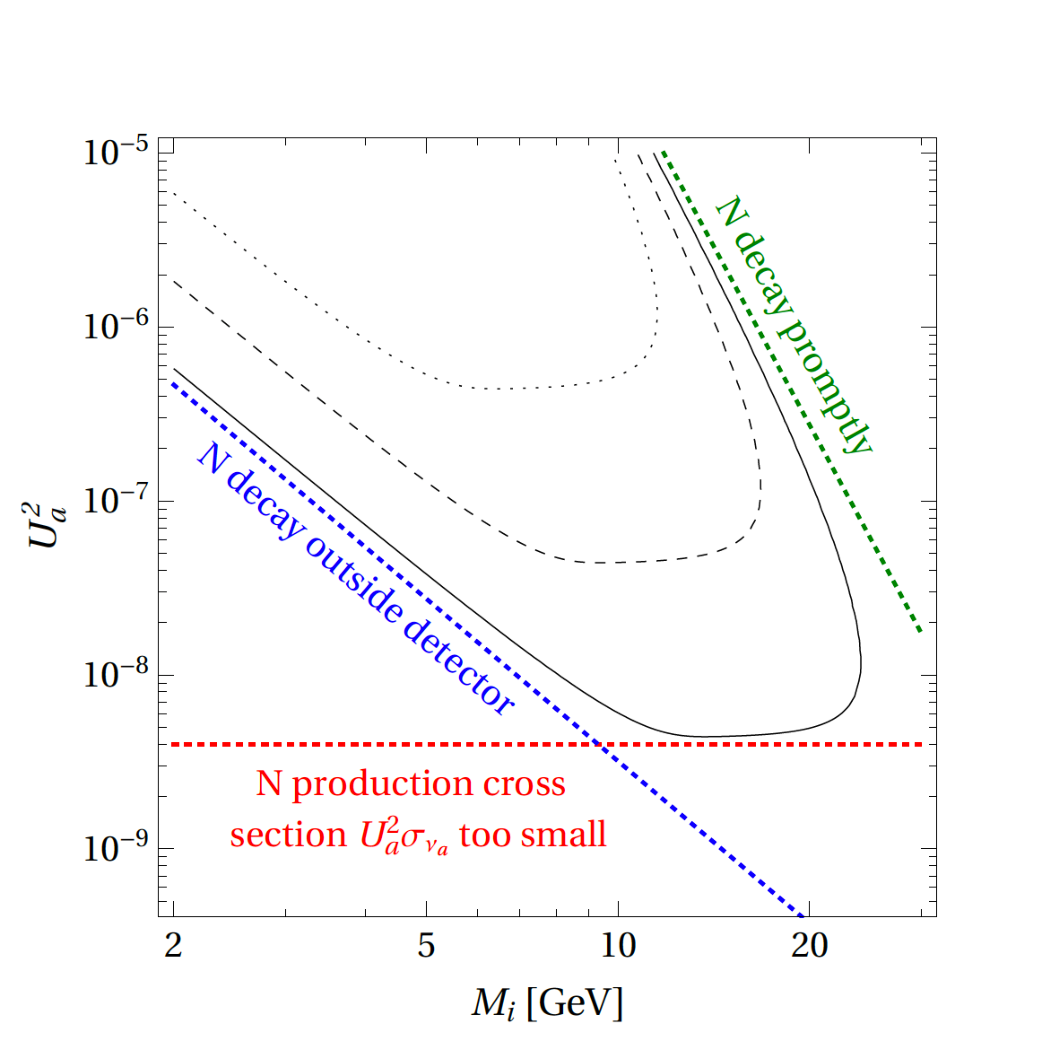
\includegraphics[clip,trim=0.cm 0cm 0cm 2cm, width=.38\textwidth]{Figures/c7/marco_god.pdf}
    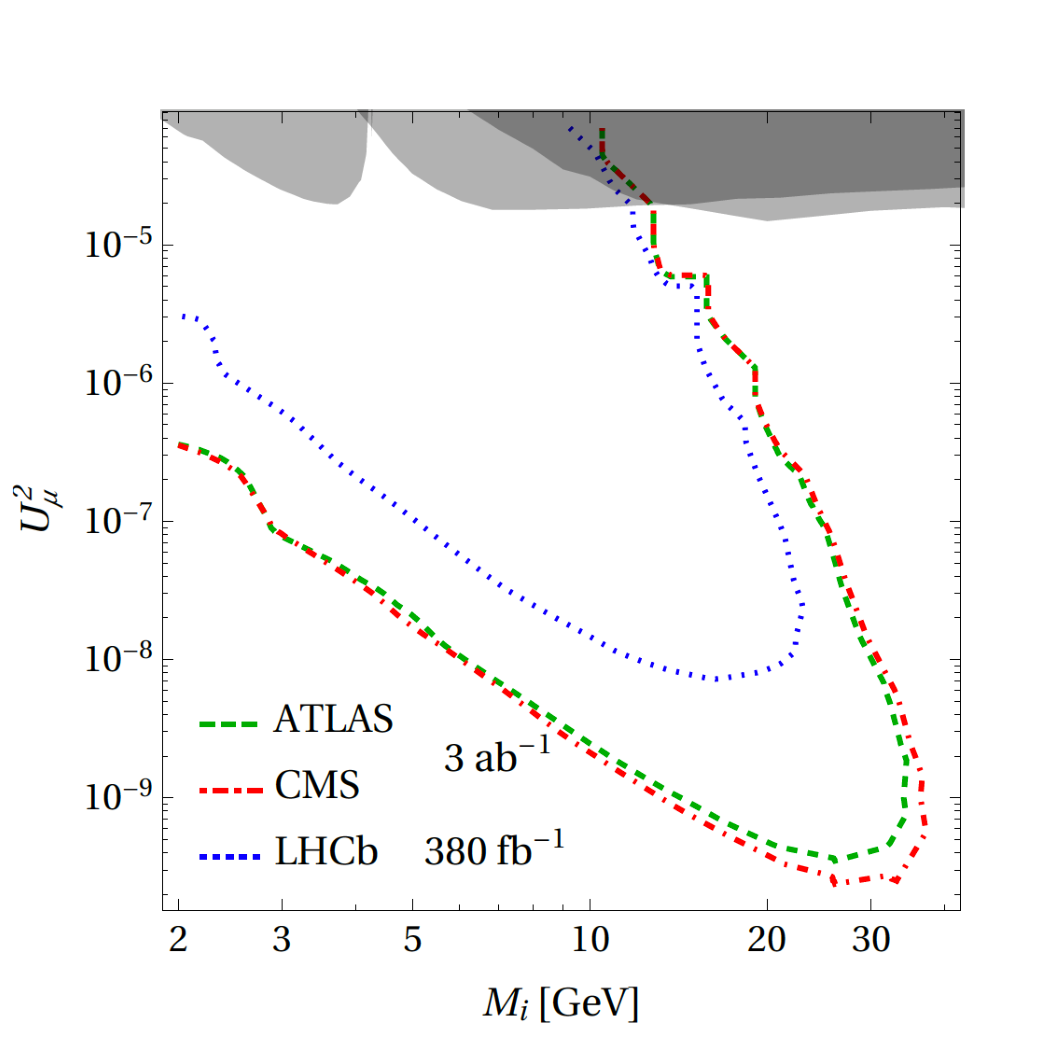
\includegraphics[clip,trim=0.cm 0cm 0cm 2cm, width=.37\textwidth]{Figures/c7/marco_mu_HL.pdf}
\caption{Left, a scheme illustrating the three main challenges in
  improving the sensitivity in a displaced analisys. Right, exclusion
  limits of ATLAS, CMS (3\abinv) and LHCb (380\fbinv)
 for the HL-LHC for \mixparm. Both plots are
  from Ref.~\cite{Drewes_2020_jan}. }
\label{fig:marco_sketch_ll}
\end{figure}


The displaced vertices
searches will profit from the programmed ATLAS and CMS detector
upgrades for the HL-LHC. 
They will increase coverage in the forward regions, they
will contribute to have better timing and spatial resolutions, and
they will add novel features like track
triggers~\cite{Alimena_2020}.\\
The subsequent brief descriptions can be extended further
in
Ref.~\cite{CERN-LHCC-2017-009,CERN-LHCC-2017-011,CERN-LHCC-2017-012,CERN-LHCC-2017-027,CERN-LHCC-2017-013}.

At the HL-LHC the
instantaneous luminosity will be a factor $\sim$5 higher than the LHC
one, with 140-200 pp collisions in each bunch crossing. This harsh
environment will make object reconstruction and particle
identification more difficult due to tracks coming from nearby
vertices making the planned detector upgrades essential. Thus, better coverage in $|\eta|$ and timing and spatial
resolution become crucial to
separate distinct events from each others. 


The CMS inner tracker will have four additional cylindrical 
layers covering the region with $|z| < $ 200 mm with the first layer positioned at
28 mm, and up to twelve endcap
disks, which will improve the $|\eta|$ coverage going from the current
value of 2.4 to almost 4 (Figure~\ref{fig:MDT_alimena}, left).
Extra modules will be installed in
the CMS outer tracker. Correlating the signals from their sensors, the modules called \pt will be able to identify
the hit pairs (named ‘stubs’) consistent with particles above \pt =
2\GeV. Furthermore these stubs are given as input to the L1 trigger, which enables the L1 trigger to make use of track-finding.

Additional muon chambers will be set up in the endcaps. They will be included in
the muon trigger at L1. The supplementary hits in the
endcap, with improved algorithms, will allow high trigger efficiency 
on displaced muon tracks regardless of the high occupancy environment of the HL-LHC.
 

The CMS MIP timing detector (MTD) will
consist in a barrel and an endcap parts formed by a single layer
module placed between the tracker
and calorimeters covering $|\eta|$ up to $\sim$3.
MTD will improve reconstruction by collecting timing information on
charged particles and by combining tracking with timing. The design will provide a timing resolution
at the start of HL-LHC of $\sim$ 30--40 ps for \pt threshold of
0.7\GeV, the timing resolution in the barrel will degrade to 50--60 ps
at end of HL-LHC~\cite{Marta}. The introduction of a timing detector will help for
the mitigation of pile-up effects
\begin{figure}[h]
\centering
    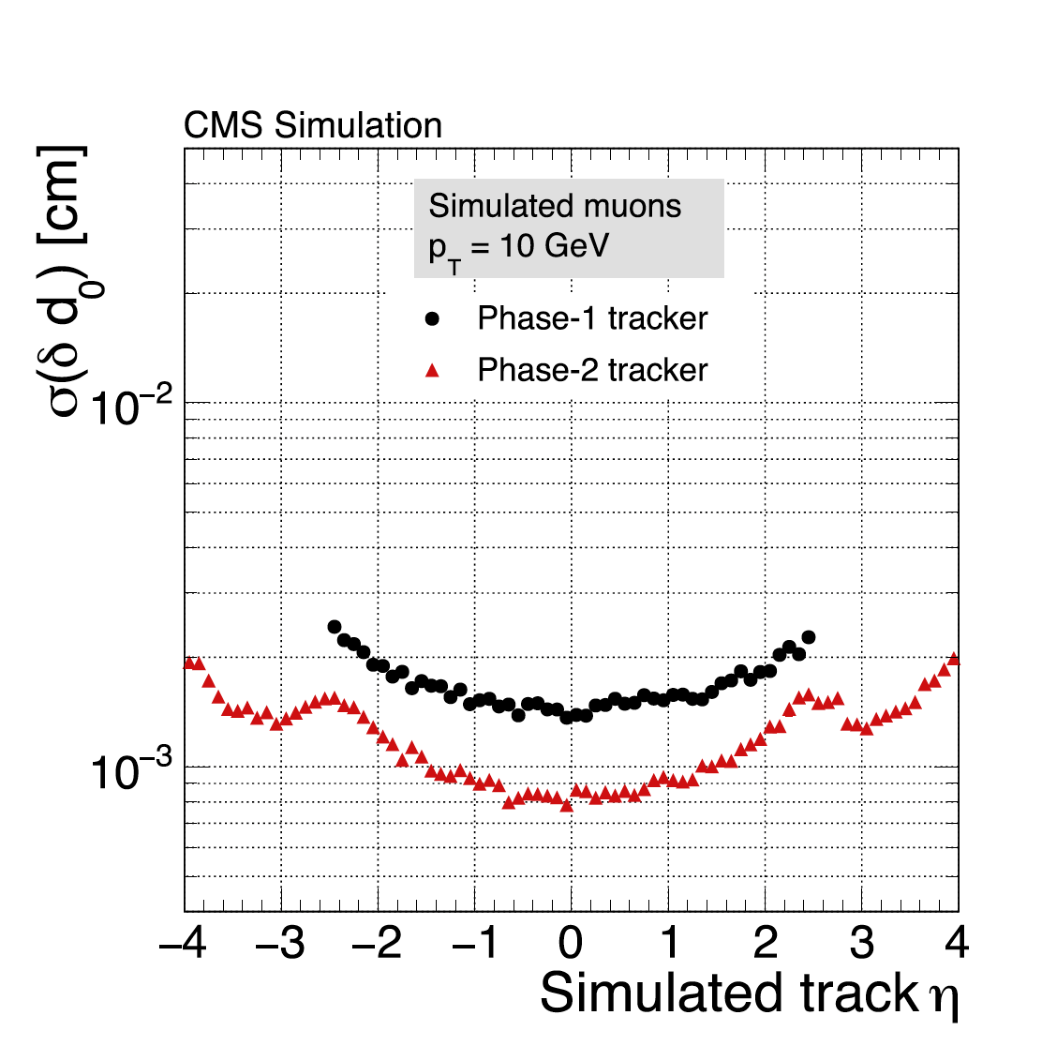
\includegraphics[clip,trim=0.5cm 0cm 0.cm 1.8cm, height =6cm]{Figures/c7/IPrel.pdf}
    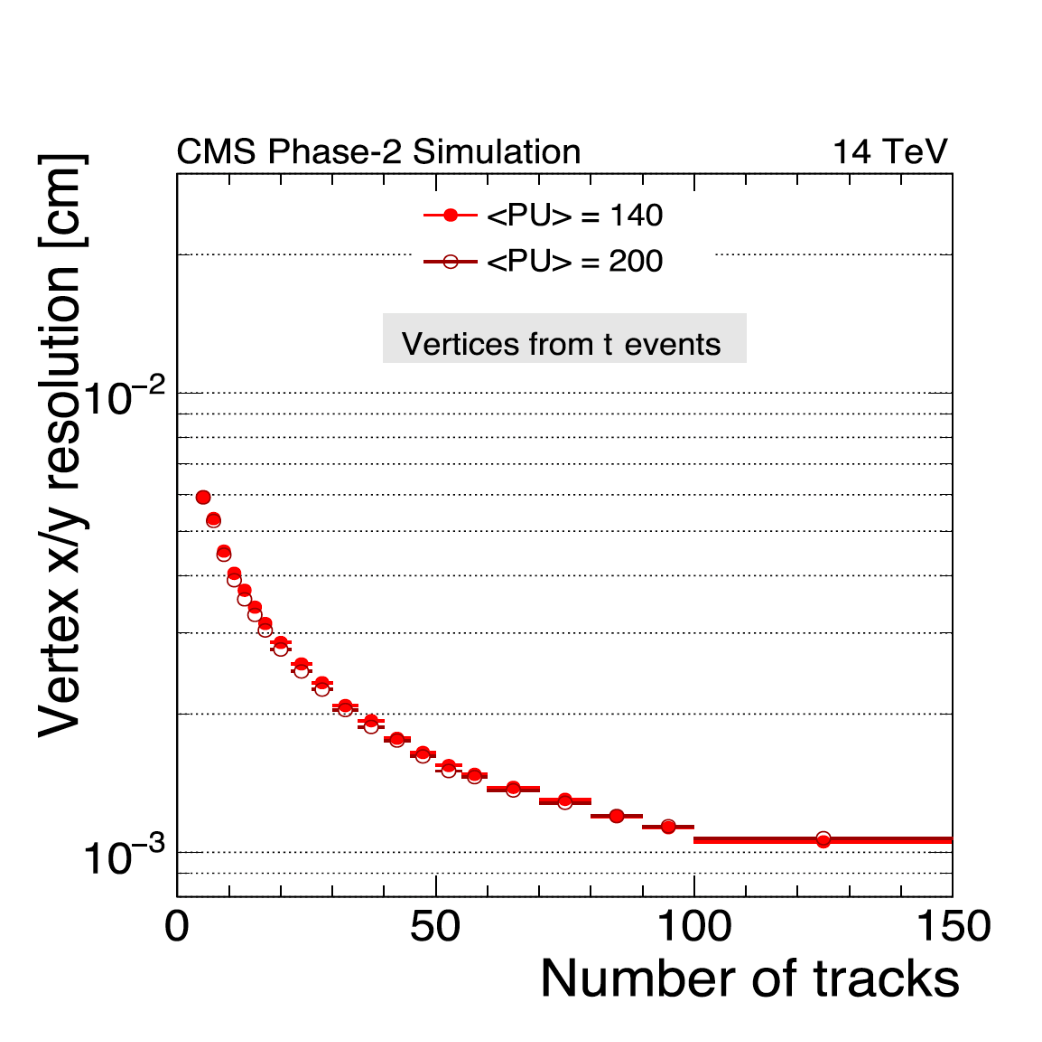
\includegraphics[clip,trim=0.5cm 0cm 0.cm 1.3cm, height = 6.3cm]{Figures/c7/vertexrel.pdf}\\
    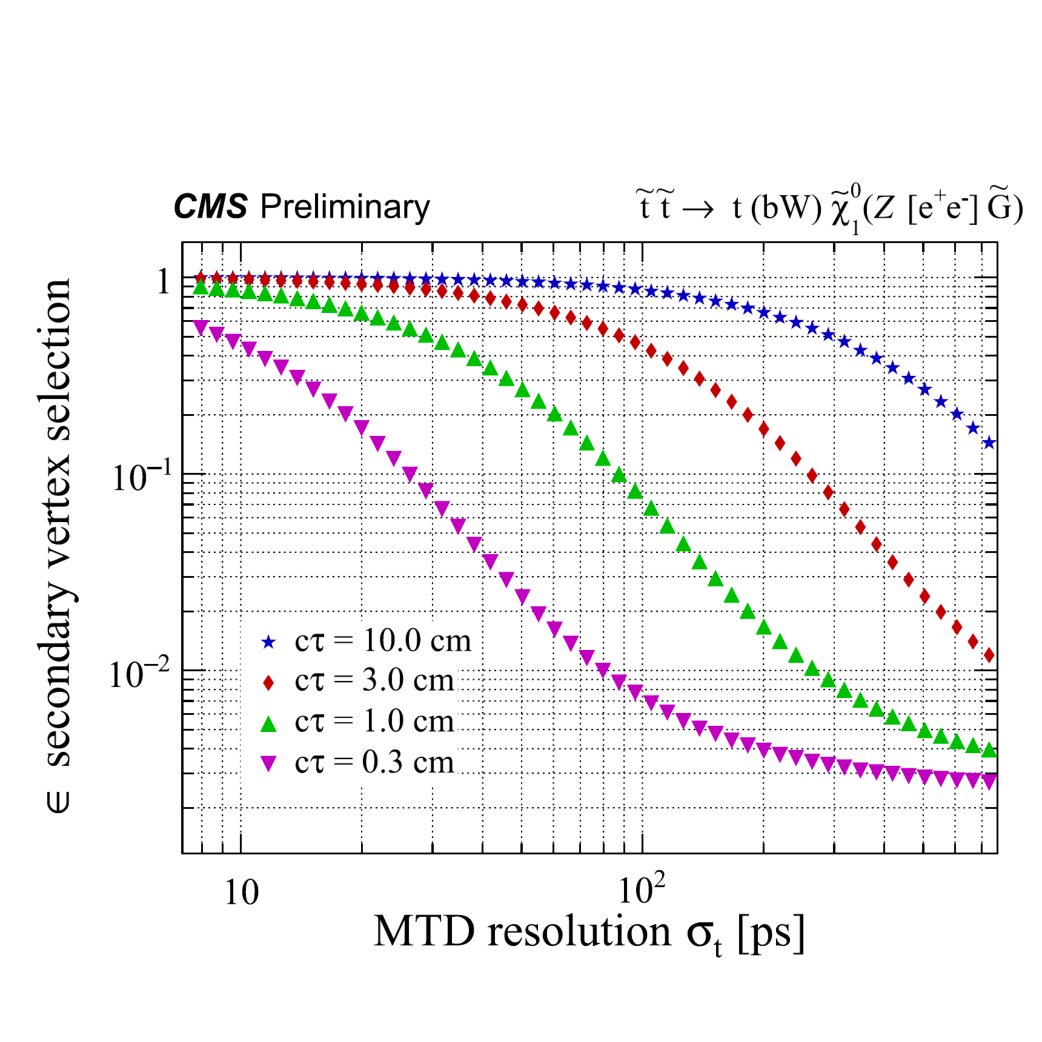
\includegraphics[clip,trim=0.5cm 1cm 0.cm 3cm, height = 6cm]{Figures/c7/MDT.pdf}
\caption{Top-left, relative resolution of the transverse impact
parameter as a function of the $\eta$ for the Run2 (black dots) and the
HL-LHC (red triangles) CMS tracker, using single isolated muons with
\pt of 10 GeV. Top-right, x and y position resolution of the vertex as a function of the
number of tracks associated to the vertex, with two pile-up scenarios. 
 Bottom, efficiency as a function of the timing
resolution of the MTD for reconstruction of a specific Supersymmetry
model considering events with a separation of
PV and SV by more than 3$\sigma$ in both space and time. All plots are
  from Ref~\cite{Alimena_2020}}
\label{fig:MDT_alimena}
\end{figure}

After exploring the CMS outlook for the next 15 years, we have to satisfy
our curiosity and look at the forthcoming experimental landscape. We
focus only on the research program for long-lived particles at the LHC,
in the specific cases designed to probe HNLs.

The \textbf{MATHUSLA} (MAssive Timing
Hodoscope for Ultra-Stable neutraL pArticles) experiment will look for
long-lived particle with $c\tau \gg$ 100 m. MATHUSLA is a
large, simple surface detector (see Figure~\ref{fig:mathu2}) able to reconstruct SVs with proper timing
resolution. The main
part is a tracker array located on top of a 200 m $\times$ 200 m
$\times$ 20 m air-filled decay volume.
The great potential of such experiment comes from the dual geometric and timing
requirements. The trajectories of particles coming from displaced
vertices are fitted to reconstruct SVs. These SVs must satisfy the rigorous
condition that all tracks coincide in time at the SV. These demanding geometric and timing
requirements make sure it is very unlikely for backgrounds to mimic
the long-lived signals.\\
MATHUSLA can excellently probe HNLs in a region of phase space close to that reachable
with present and future fixed-target experiments like SHiP or
DUNE. The derived sensitivity is shown in Figure~\ref{fig:mathu2} under
the plausible assumption of zero background. Comparing with CMS and
ATLAS projections, it is foreseen that MATHUSLA results will have rather
better sensitivity than the main LHC detectors for those HNL mass
regimes that suffer from triggering and reconstruction restrictions.
\begin{figure}[h!]
\centering
    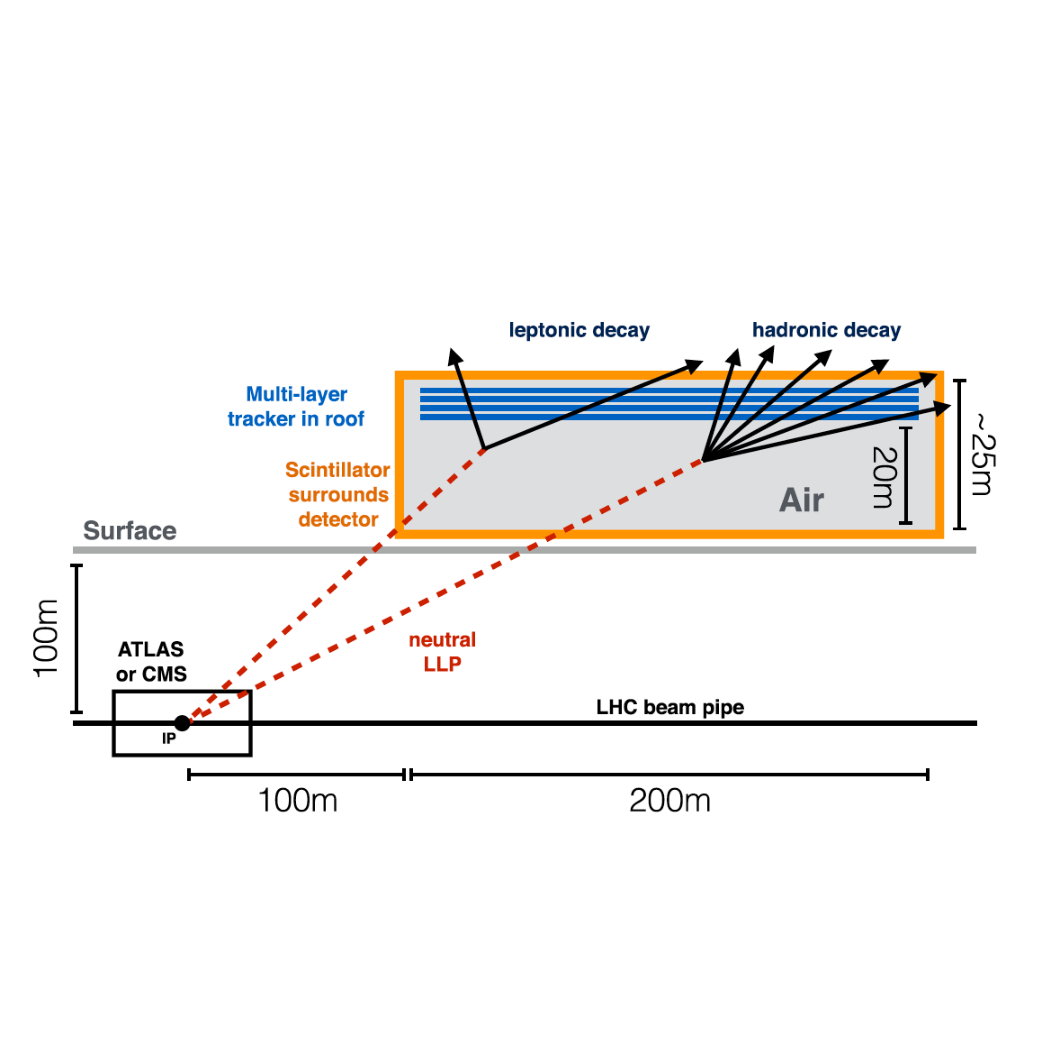
\includegraphics[clip,trim=0.3cm 0cm 1.cm 2cm, width=.45\textwidth]{Figures/c7/mathusla1.pdf}
    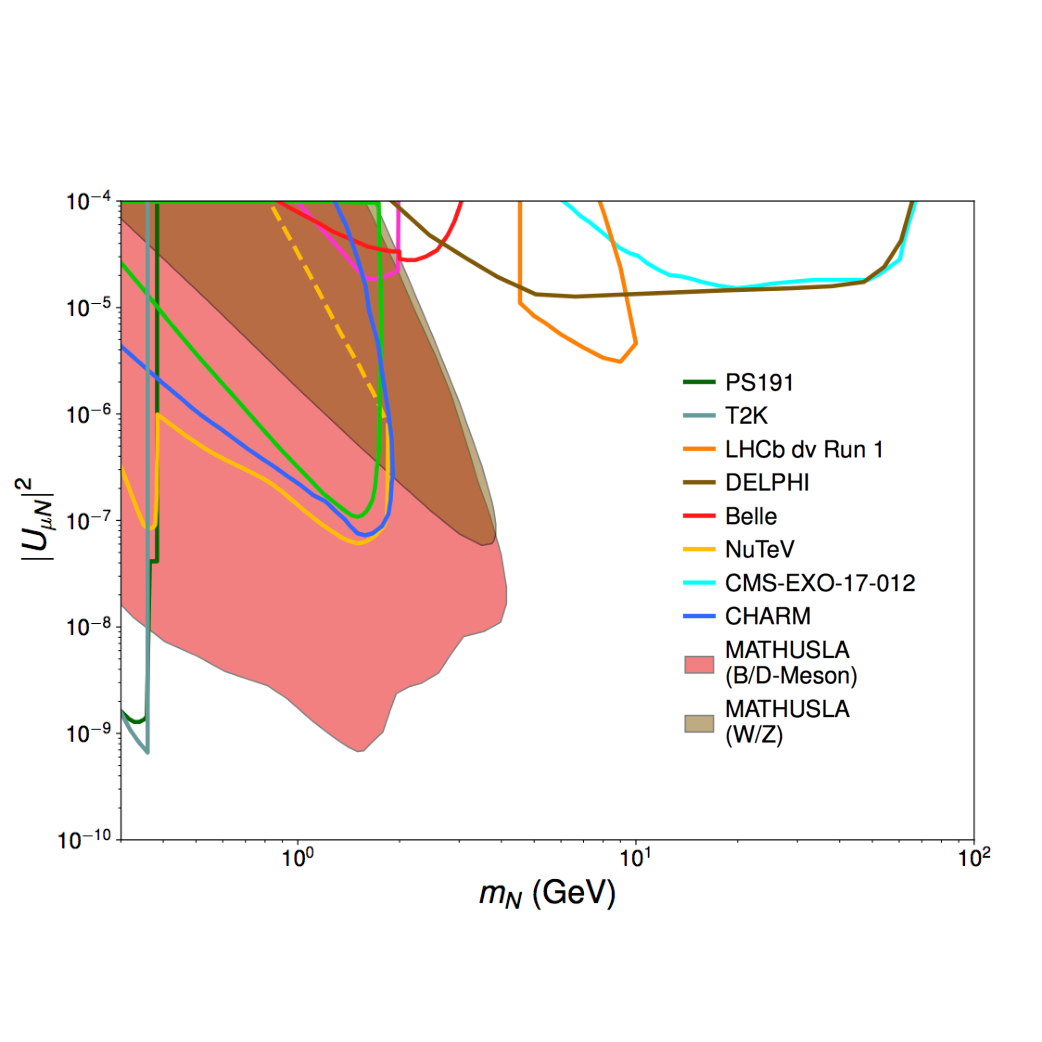
\includegraphics[clip,trim=0cm 2cm 0.5cm 3cm, width=.54\textwidth]{Figures/c7/mathusla2.pdf}
\caption{Left, simplified MATHUSLA detector
  layout~\cite{Alimena_2020}. Right, projected sensitivity in \mixparm
  - $m_\hnl$ plane for \hnl produced in W/Z decays (brown regions) and in B/D-meson decays (light red region)~\cite{Curtin_2019}.
}
\label{fig:mathu2}
\end{figure}

%The \textbf{CODEX-b} (COmpact Detector for EXotics at LHCb) experiment
%will be placed in the LHCb cavern 25 m far from the interaction point
%and shielded by 3 m thick wall made of concrete. The initial design
%will be a 10 m $\times$ 10 m
%$\times$ 10 m volume with RPC tracking layers.\\

In the central regions of Figures~\ref{fig:HNL_bc6_pbc_2}
and~\ref{fig:HNL_bc7_pbc_2}, there are striking exclusion curves
labeled ``SHiP''. They are obtained by taking into account the reach of
the general purpose fixed target experiment projected at the CERN SPS
accelerator, \textbf{SHiP} (Search for Hidden Particles)~\cite{bonivento2013proposal,
  shipcollaboration2015facility}. Although it has been decided to
conclude the preparation and to terminate the project of the facility,
it is interesting to give a brief description of the possible
contributions it could have given to the HNL hunt.\\
The principal physics objectives consist of probing SM extensions
which include very weakly and long-lived particles by directly
detecting their decays to SM particles.
\begin{figure}[h!]
\centering
    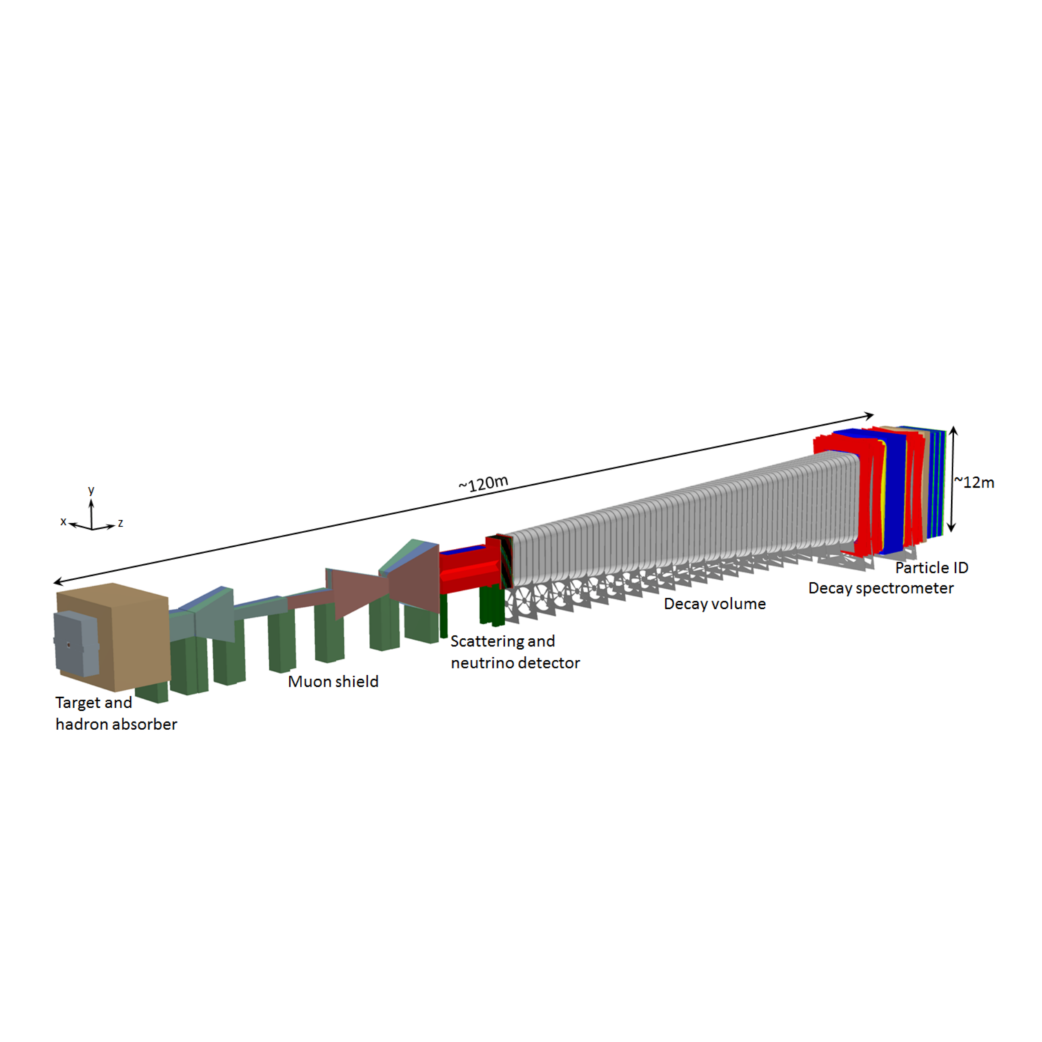
\includegraphics[clip,trim=0.3cm 5cm 1.cm 7cm, width=.75\textwidth]{Figures/c7/ship.pdf}
\caption{Schematic overview of the SHiP experiment~\cite{CERN-SHiP-NOTE-2018-001}.
}
\label{fig:ship1}
\end{figure}
In the forward region of the SHiP detector a big and powerful 
magnetic shield is located conceived to remove all charged particles
coming from the beam-target collision. Two complementary
parts follow: the ``Scattering and Neutrino
Detector (SND)'', and the ``Hidden Sector (HS)
spectrometer''~\cite{CERN-SHiP-NOTE-2018-001}. The HS is designed to
measure the decays of long-lived particles by reconstructing the
SVs. The decays happen in a 50 m long empty decay volume located
between SND and HS. The HS is equipped with 
tracker, timing, calorimeter and muon detectors. \\
For HNL mass scenarios $<2$\GeV, SHiP would have improved the sensitivity
with respect to previous searches~\cite{bonivento2013proposal}.\\
The projections are done considering \mixparm, assuming HNL decays $\hnl
\rightarrow \mu^{-} \pi^{+}$ and using $D
\rightarrow \mu^{+} \hnl X$ as production mechanism. The calculations
led to the conclusion that for a $m_\hnl = 1$\GeV SHiP would record
120 reconstructed $\hnl
\rightarrow \mu^{-} \pi^{+}$ using as parameters \mixparm $= 10^{-8}$,
$c\tau = 1.8 \times 10^{-4}$~\cite{bonivento2013proposal}. \\

In the CERN North-Area in Prevessin, we find not only SHiP but also the
\textbf{NA62}~\cite{Gil_2017} experiment which significantly contributes in
the HNL hunt. Using data 
collected during the first physics data-taking in 2015, the NA62
Collaboration published a search for $K^{+} \rightarrow \hnl \ell^{+}$
decays for $170 <m_\hnl< 448$ MeV$/c^{2}$~\cite{Cortina_Gil_2018} (the
results are shown in Figure~\ref{fig:HL_alimena}). The analyzed events
were collected by NA62 in 2015 at $\sim$1\% of the nominal designed
beam intensity.\\
During Run3, NA62 is planning to run in beam dump mode with
nominal beam intensity of $10^{18}$ pot (proton on target). With these
conditions the final exclusion sensitivity will be improved with 
respect to CHARM limits (Figures~\ref{fig:HNL_bc6_pbc_2}
and~\ref{fig:HNL_bc7_pbc_2})
by about one order of magnitude in similar phase
space~\cite{na62Drewes_2018}.
The projections are done assuming zero background and 
correspond to the 90\% CL for \hnl decaying into at least two
 charged tracks. The full study can be found in
 Ref~\cite{na62Drewes_2018} and the estimated limits in Figures~\ref{fig:HNL_bc6_pbc_2}
and~\ref{fig:HNL_bc7_pbc_2}. The authors consider NA62 to be one of
the world’s best experiment to look for HNLs with masses in the range
delimitated by those of kaons and D-mesons~\cite{na62Drewes_2018}.\\
\begin{figure}[h]
\centering
    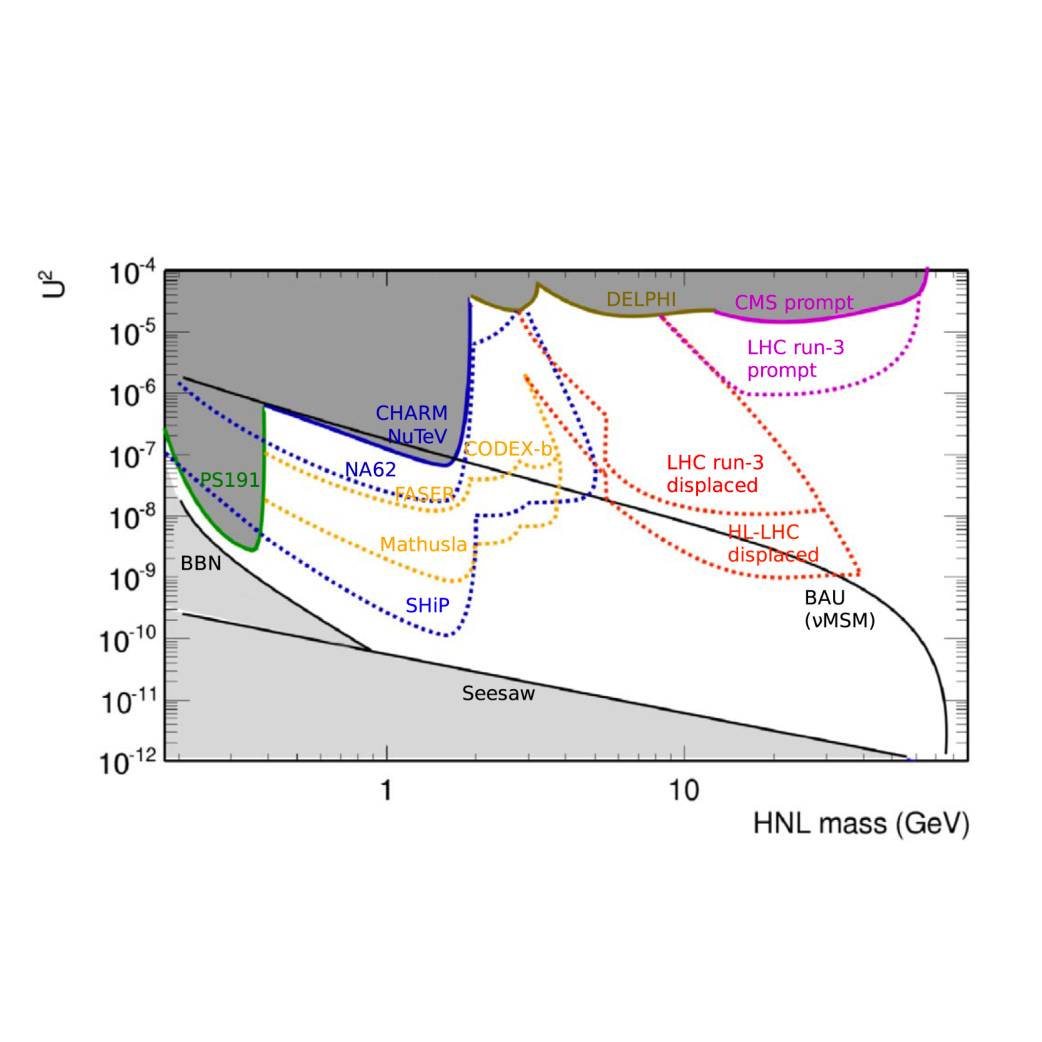
\includegraphics[clip,trim=0.5cm 3.5cm 1.cm 4.3cm, width=.78\textwidth]{Figures/c7/projection_alimena.pdf}
\caption{``Summary of projected experimental sensitivities to HNLs in various
experiments, in the coupling strength \mixpar versus mass
plane. The projections labelled ``LHC Run 3'' and ``HL-LHC'' are for HNLs in \PW decays
in general-purpose experiments, and the one labelled ``Mathusla'' assumes the full HLLHC
MATHUSLA dataset. The estimated sensitivity will reach the upper theoretical
constraint (labeled ``BAU'') in the Neutrino Minimal Standard Model
for accounting for baryon asymmetry in the Universe
while the lightest HNL is a dark-matter
candidate''~\cite{PhysRevD.87.093006}. Plot from Ref.~\cite{Alimena_2020}}
\label{fig:HL_alimena}
\end{figure}

Before wrapping up, it is worth mentioning the projections for
HL-LHC. In Figure~\ref{fig:HL_alimena} the exclusion reach using Run3
and 3\abinv (HL-LHC) data is shown for long-lived HNL analysis
performed at CMS or ATLAS. 

Quite far in future, the next breakthrough moment will happen with the
dedicated searches at high energy electron-positron circular collider,
FCC-ee. A first exploratory study about HNL sensitivities shows exclusion limits
down to \mixpar $\simeq 10^{-12}$ covering \hnl masses between 10 and
80 \GeV$/c^2$~\cite{blondel2014search}. The estimations are obtained
considering $\PZ \rightarrow \nu \hnl$ decays with \hnl further
decaying into
$\hnl \rightarrow mu^{+} W^{-} \rightarrow mu^{+}
q\bar{q}$. Long-lived HNL scenarios are examined with decay length
going from 0.01 cm up to 500 cm~\cite{blondel2014search}.\\


This final chapter is not expected to cover all the existing projections and all the new
experiments. 
Instead, the outlook tries to give a feeling of the vast landscape
where the two CMS HNL searches sit. The idea is to give sense of the
context and of the perspective from where to look these results
from. \\
We have briefly seen the potential of the planned CMS detector
upgrades, of the new triggers, of the improved reconstruction algorithms and analysis strategies that
have been further developed. \\
The very wide range of masses, energies and models necessitates to
explore the complementary reach of the current and future experiments.\\
During the five years of my PhD, it has become so clear that collaborations
among the LHC experiments, the theorists and the next generation of
facilities is essential to a comprehensive
understanding of the heavy neutral lepton frontier and to not missing
new physics potential in the upcoming era of the HL-LHC.

















%%%%%%%%%%%%%%%%%%%%%%





